\documentclass[10pt, compress]{beamer}

\usetheme{m}

%\usetheme{metropolis}
%\usepackage{xspace}

\usepackage{booktabs}
\usepackage[scale=2]{ccicons}
\usepackage{minted}
\usepackage{listings}

\usetikzlibrary{calc}
\usetikzlibrary{positioning}
\usetikzlibrary{shapes.geometric}
\usetikzlibrary{arrows}
\usetikzlibrary{matrix,positioning,calc,fit}
\usetikzlibrary{chains, positioning, shapes, arrows}
\graphicspath{ {images/} }
\usefonttheme[onlymath]{serif}
\usetikzlibrary{matrix,positioning,calc,fit}

\tikzset{circ/.style={draw,circle,node distance=2mm,inner sep=0.1pt},topath/.style={to path={|-(\tikztotarget)}}}

\lstset{
  basicstyle=\ttfamily\tiny
  %extendedchars=true,
  %breaklines=true,
  %frame=lrtb,
  showspaces=false,
  showtabs=false,
  language=C, 
  moredelim=[is][\underbar]{_}{_},
  keepspaces=true
  %xleftmargin=10pt,
  %xrightmargin=5pt,
  %framexleftmargin=5pt,
  %framexrightmargin=-1pt,
  %framexbottommargin=4pt,
}

\usemintedstyle{trac}

\title[Performance evaluation of NLFSR enumeration]{Performance evaluation of NLFSR enumeration on heterogeneous environments}

\subtitle{New List of Maximum Period NLFSRs}

\date{\today}
\author{Paweł Augustynowicz, Krzysztof Kanciak, \underline{Janusz Szmidt}}
\institute[shortinst]{Faculty of Cybernetics, Military University of Technology, Warsaw\\
Military Communication Institute, Department of Cryptology, Zegrze}

\begin{document}

\maketitle

\begin{frame}{Binary Feedback Shift Register - FSR}
Let $ \mathbb{F}_2 $ be a binary field and $ \mathbb{F}^{n}_2 $ the $ n $-dimensional vector space over $ \mathbb{F}_2 $.
Let us consider a mapping \ \ $ \mathfrak{F}: \mathbb{F}^{n}_2\rightarrow\mathbb{F}^{n}_2 $ \ \
of the form
\[ \mathfrak{F}(x_0, \ldots , x_{n-1})=(x_1, x_2, \ldots , x_{n-1}, f(x_0, \ldots , x_{n-1})), \ \ \ \ \ \ \ (1) \]
where $f$ is a Boolean function of $n$ variables of the form
\[ f(x_0, \ldots , x_{n-1})=x_0 + F(x_1, \ldots , x_{n-1}),  \]
and $ F $ is a Boolean function of $ n-1 $ variables. \\
The formula (1) defines a nonsingular \textit{FSR} of order $ n $. \\
A nonsingular register decomposes the space  $ \mathbb{F}^{n}_2 $ into a finite number of disjoint cycles.
\end{frame}

\begin{frame}
\frametitle{The generation of binary sequences}
\begin{itemize}
\item Let us consider the binary sequence $ \textbf{s} = (s_{0}, s_{1}, \ldots ) $, which $ n $-initial elements $ (s_{0}, \ldots , s_{n-1}) $ are given and the next elements are calculated from the formula
\[s_{i+n} = f(s_{i}, s_{i+1}, \ldots , s_{i+n-1}) 
= s_i + F(s_{i+1}, \ldots , s_{i+n-1}) \ \ \ for  \ \ i \geq 0 .\]
\item In particular we have the linear recurrence
\[ f(x_{0}, x_{1}, \ldots , x_{n-1}) = x_{0} +  c_{1}x_{1} + \ldots + c_{n-1}x_{n-1}. \]
and the corresponding \textit{LFSR.}
\item  \emph{The Algebraic Normal Form (ANF)} of a Boolean function $ f $ of $ n $ variables is given by
\[f(x_{0}, x_{1}, \ldots , x_{n-1})=\sum a_{i_{1}, \ldots , i_{t}} x_{i_{1}} \cdots x_{i_{t}} , \ \ a_{i_{1}, \ldots , i_{t}} \in \mathbb{F}_{2} ,\]
where the sum is over all  $ t $-subsets $ \{ i_{1}, \ldots , i_{t} \} \subset \{0, 1, \ldots , n-1 \}.$
\end{itemize}
\end{frame}

\begin{frame}{De Bruijn sequences}
\begin{itemize}
\item If it is only one cycle (its length is $ 2^n $), then we have de Bruijn sequence.
\item The number of all non-equivalent de Bruijn sequences of order $ n $ is equal to
\[ B_{n} = 2^{2^{n-1}-n} \]
\item The number of deBruijn sequences grows double-exponentially:
\[ n = 4, \ \ \ B_4 = 2^4 = 16 \]
\[ n = 5, \ \ \ B_5 = 2^{11} = 2048 \]
\[ n = 6, \ \ \ B_6 = 2^{26} = 67,108, 864 \]
\[ n = 7, \ \ \ B_7 = 2^{55} \] 
\end{itemize}
\end{frame}

\begin{frame}{Linear modified de Bruijn - period ${2^n - 1}$}
\begin{itemize}
\item Let \   $p(x) = x^{n} + c_{n-1}x^{n-1} + \dots + c_{1}x + 1 $ \
be a primitive polynomial of degree $ n $ with binary coefficients.
\item Then the linear recurrence
\[g(x_{0}, x_{1}, \ldots , x_{n-1}) = x_{0} + c_{1}x_{1} + \dots + c_{n-1}x_{n-1} \]
generates the $ m$-sequence which is a binary sequence of the period $ 2^n-1. $
\item The polynomial $p(x) $ is called the characteristic polynomial of the generated $m$-sequence.
\item The number of $m$-sequences of order $n$ is equal to 
\[ \frac{\phi (2^n-1)}{n}   \]
\end{itemize}
\end{frame} 

%\iffalse
\begin{frame}{An example of LFSR of order n = 16}

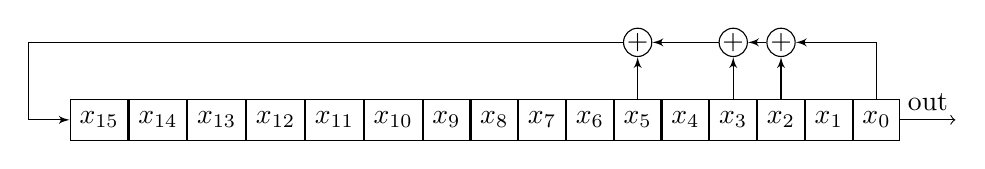
\begin{tikzpicture}[start chain=1 going left,
    start chain=2 going left,]
  \tikzstyle{abox}=[draw,minimum width=1.5em,minimum height=1.5em]
  \tikzstyle{acircle}=[draw,circle,minimum size=1em,inner sep=0pt]
  \tikzstyle{boxchain}=[node distance=0pt]
  \tikzstyle{arrowline}=[draw, -latex']
  \def\chainshift{7em}
  \def\connectionsep{1.5em}

  \begin{scope}[boxchain]
    \node [on chain=1, abox] (ch1a0) {$x_{0}$};
    \node [on chain=1, abox] (ch1a1) {$x_{1}$};
    \node [on chain=1, abox] (ch1a2) {$x_{2}$};
    \node [on chain=1, abox] (ch1a3) {$x_{3}$};
    \node [on chain=1, abox] (ch1a4) {$x_{4}$};
    \node [on chain=1, abox] (ch1a5) {$x_{5}$};
    \node [on chain=1, abox] (ch1a6) {$x_{6}$};
    \node [on chain=1, abox] (ch1a7) {$x_{7}$};
    \node [on chain=1, abox] (ch1a8) {$x_{8}$};
    \node [on chain=1, abox] (ch1a9) {$x_{9}$};
    \node [on chain=1, abox] (ch1a10) {$x_{10}$};
    \node [on chain=1, abox] (ch1a11) {$x_{11}$};
    \node [on chain=1, abox] (ch1a12) {$x_{12}$};
    \node [on chain=1, abox] (ch1a13) {$x_{13}$};
    \node [on chain=1, abox] (ch1a14) {$x_{14}$};
    \node [on chain=1, abox] (ch1a15) {$x_{15}$};
  \end{scope}

  \path[->] (ch1a0) edge node[above] {out} +(1,0);
  \node [acircle,above=\connectionsep of ch1a2] (p-ch1a2) {$+$};
  \node [acircle,above=\connectionsep of ch1a3] (p-ch1a3) {$+$};
  \node [acircle,above=\connectionsep of ch1a5] (p-ch1a5) {$+$};
 
  \path [arrowline] (ch1a2) -- (p-ch1a2);
  \path [arrowline] (ch1a3) -- (p-ch1a3);
  \path [arrowline] (ch1a5) -- (p-ch1a5);
  \path [arrowline] (ch1a0) --(p-ch1a2-|ch1a0) |- (p-ch1a2);
  
  \path [arrowline] (p-ch1a2) -- (p-ch1a3);
  \path [arrowline] (p-ch1a3) -- (p-ch1a5);

  \path [arrowline] (p-ch1a5) -- ([xshift=-1.5em]p-ch1a5-|ch1a15.west) |- (ch1a15.west);
\end{tikzpicture}

The device realizing an LFSR of order 16 given by the recurrence
\[ x_0 + x_2 + x_3 + x_5 \]
and the corresponding primitive characteristic polynomial
\[x^{16}+x^{5}+x^{3}+x^{2}+1 \]
The period of the generated binary sequence is $2^{16} - 1. $ \\
The theory of LFSRs is well understood, but that for NLFSRs (Nonlinear Feedbach Shift Registers) is far to be complete.
\end{frame}
%\fi

%We can say that LFSRs are very mature and all problems related to LFSRs are solved. 
%It is known that $n$-bit LFSR has the maximum period of $2^{n}-1$ if and only if its characteristic polynomial of degree $n$ is primitive.
%No such rule for NLFSRs has been found so far. 
%It has to be pointed that despite many LFSRs applications (stream ciphers, pseudorandom number generators, error detection and correction, data compression) their pseudorandom sequences are not cryptographically secure. 
%Only $2n$ consecutive bits of LFSRs sequence is enough to deduce $n$-bit LFSR structure. by using a Berlekamp-Massey algorithm. 

\iffalse 
\begin{frame}[fragile]
\frametitle{LFSR example}
\begin{columns}
\column{0.7\textwidth}
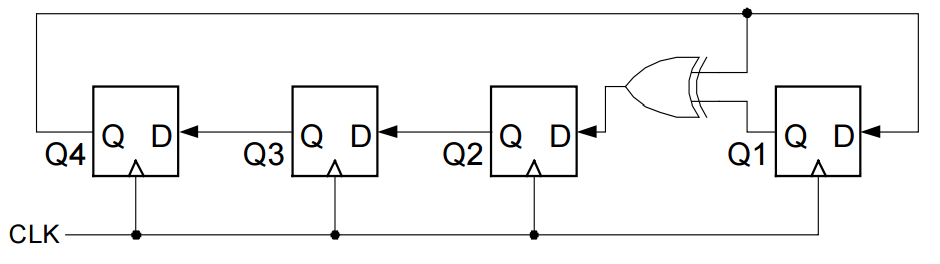
\includegraphics[scale=0.3]{galex}
\column{0.3\textwidth}
feedback function $x^4+x+1$\\
bit pattern $11001$
\end{columns}
\begin{columns}
\column{0.5\textwidth}
\begin{lstlisting}
0:  _0001_0
xor 00000
1:  0_0010_0 
 xor 00000
2:   0_0100_0
  xor 00000
3:    0_1000_0
   xor 10011
4:     0_0011_0
    xor 00000
5:      0_0110_0
     xor 00000
6:       0_1100_0
      xor 10011
7:        0_1011_0
....
\end{lstlisting}
\column{0.5\textwidth}
$\alpha^0=1$\\
$\alpha^1=x$\\
$\alpha^2=x^2$\\
$\alpha^3=x^3$\\
$\alpha^4=x^4 mod(x^4+x+1)=x+1$\\
$\alpha^5=x^2+x$\\
$\alpha^6=x^3+x^2$\\
$\alpha^7=x^3+x+1$
\end{columns}
$n$-bit LFSR has the maximum period of $2^{n}-1$ iff its characteristic polynomial of degree $n$ is primitive.
\end{frame}

%Existing methods of cryptanalysis do not provide any efficient algorithm to deduce the structure of NLFSRs by only generated sequences which makes NLFSRs much more appealing for cryptographers. 
%In recent years, NLFSRs have received much attention in designing many cryptographic algorithms such as stream ciphers \cite{EPRINT:ZhaWan09a}, kdfs (KATAN lightweighht block cipher),  lightweight block ciphers and sponge-based generators. 
%GRAIN which is NIST standard, eStream competition winner
%Sequences generated by full period NLFSRs are also known as de Bruijn sequences. 
\begin{frame}{NLFSR example}
\begin{columns}
\column{0.5\textwidth}
$f(x_0, x_1, x_2) = 1 + x_0 + x_1 + x_1x_2$

\begin{tabular}{ |c|c|c|c } 
\hline
$i$ &  $(x_i, x_{i+1}, x_{i+2})$ & $x_{i+3}$ \\
\hline
1 & 001 & 1 \\ 
2 & 011 & 1 \\ 
3 & 111 & 0 \\ 
4 & 110 & 1 \\ 
5 & 101 & 0 \\ 
6 & 010 & 0 \\ 
7 & 100 & 0 \\ 
\hline
\end{tabular}
\column{0.5\textwidth}
\begin{itemize}
    \item Sequences generated by full period NLFSRs are known as de Bruijn sequences
    \item In a de Bruijn sequence of order $n$ all $2^n$ different binary $n$-tuples appear exactly once
    \item It is known that the number of different de Bruijn sequences of order $n$ is equal to $2^{2^{n-1}-n}$
    \item Existing methods do not provide any efficient algorithm to deduce the structure of NLFSRs by only generated sequences
\end{itemize}
\end{columns}
\end{frame}

%Feedback shift registers (FSR) are used to generate binary sequences which can be applied in cryptographic systems. 
%Especially stream ciphers usually use FSRs to construct invertible mappings to prevent reduction of the entropy of the internal state of a cipher. 
%The strongly desirable property is a long period of FSR. 
%The period of a mapping is the length of the longest cycle in its state transition graph. 
%For cryptographic aplications, it is needed to prevent FSR based mapping sequence of generated states to be trapped in short cycle.
%FSRs most important advantages are high speed and low power consumption. 
%These are crucial factors for hardware cryptographic systems especially for growing market of IoT use cases. 
%Stream ciphers built on FSRs supports very high data rates, throughput and remains power efficient.
\fi

\begin{frame}{LFSR properties}
Feedback shift registers (FSR) are used to generate binary sequences which can be applied in cryptographic systems.
\vspace{1em}
\begin{columns}
\column{0.5\textwidth}
LFSRs properties:
\begin{itemize}
    \item long period equal to $2^n-1$
    \item good statistical properties
    \item easy hardware and software imeplementation
    \item high speed and low power consumption, high data rates, throughput
\end{itemize}
\column{0.5\textwidth}
but:
\begin{itemize}
    \item predictable - $2n$ consecutive bits sequence is enough to deduce LFSR structure
    \item breaking linearity with filtration function, irregular LFSRs clocking, ...and using NLFSR
\end{itemize}
\end{columns}
The problem is that the efficient method of construction cryptographically strong NLFSRs remains unknown.
\end{frame}

\begin{frame}{Experimental Setup}
% the size of chunk of data for GPU was 10000 \times 1024 whereas for CPU it was 16 \times number of cores
To estimate the performance of NLFSR enumeration we setup following experiments:
\begin{description}
\item[for GPU and FPGA] we measure the cycle enumeration time of $10^{5} \cdot 2^{10}$ of possible NLFSRs for different length of NLFSRs ($10^{5} \cdot 2^{10}$ is multiple of numbers of CUDA cores for every card that we have tested);
\item[for CPU] we measure the cycle enumeration time of $2^{14} \times number \ of \ cores$ of possible NLFSRs for different length of NLFSRs;
\end{description}
\end{frame}


\begin{frame}{GPU and FPGA Performance}
\begin{table}[]
    \centering
\begin{tabular}{ ||c||c|c|c||c|c|| } 
\hline
$n$ &  Tesla P100 & Tesla K80 & 1080GTX & Cyclone V & Stratix V\\
\hline
\hline
23 & 34    & 86    & 38   & ---   & ---   \\ 
24 & 82    & 303   & 87   & ---   & ---   \\ 
25 & 193   & 479   & 205  & ---   & ---   \\ 
26 & 425   & 991   & 408  & 1271  & 157   \\ 
27 & 818   & 2128  & 800  & 2652  & 316   \\ 
28 & 1575  & 5739  & 1639 & 5886  & 649   \\ 
29 & 3107  & 7672  & 3250 & 10526 & 1351  \\
30 & 6411  & ---   & 6576 & 21913 & 2767  \\
31 & 27817 & ---   & ---  & 51130 & 5557  \\
32 & ---   & ---   & ---  & ---   & 11773 \\
\hline
\end{tabular}    
\caption{A search time [s] for different GPUs and different length of NLFSRs.}
\label{tab:my_label}
\end{table}
\end{frame}

\begin{frame}{CPU Performance}
\begin{table}[]
    \centering
\begin{tabular}{ ||c||c|c|c|| } 
\hline
$n$ & i7-6700  & Xeon2699v3 & Xeon2699v4 \\
%\hlinealse
\hline
23 & 0,0001 & 0,0001 & 0,0002 \\ 
24 & 0,0002 & 0,0002 & 0,0003 \\ 
25 & 0,0004 & 0,0004 & 0,0007 \\ 
26 & 0,0008 & 0,0008 & 0,0014 \\ 
27 & 0,0016 & 0,0017 & 0,0027 \\ 
28 & 0,0033 & 0,0033 & 0,0055 \\ 
29 & 0,0065 & 0,0066 & 0,0110 \\
30 & 0,0130 & 0,0132 & 0,0220 \\
31 & 0,0261 & 0,0263 & 0,0439 \\
32 & 0,0546 & 0,0527 & 0,0877 \\
33 & 0,1089 & 0,1079 & 0,1753 \\
34 & 0,2179 & 0,2162 & 0,3507 \\
\hline
\end{tabular}    
\caption{A search time [s] for different CPUs and different length of NLFSRs.}
\label{tab:my_label}
\end{table}
\end{frame}



\begin{frame}{CPU vs GPU vs FPGA}
Performance of computations for CPU, GPU and FPGA was estimated by number of basic operations (feedback function evaluation) for unit per one second.
\begin{figure}[ht]
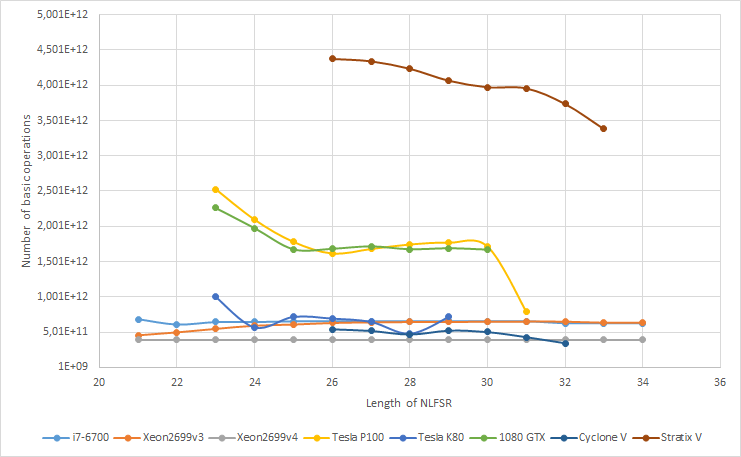
\includegraphics[width=\textwidth]{images/enumeration_fpga.png}
%[width=\textwidth,height=\textheight,keepaspectratio]
\end{figure}
\end{frame}

\iffalse

\begin{frame}{FPGA Performance}
    
\end{frame}

\begin{frame}{Conclusions}
    \begin{itemize}
        \item 
    \end{itemize}
\end{frame}

\fi 

%The problem is that the efficient method of construction cryptographically strong NLFSRs remains unknown.
%The most important NLFSR related problem is finding a systematic procedure for constructing NLFSRs with a guaranteed long period. Available algorithms either consider some special cases, or are applicable to small NLFSRs only, or produce NLFSRs which are not cryptographically strong \cite{EPRINT:DLRS13} \cite{EPRINT:Dubrova11}, \cite{EPRINT:RSWZ12}.
%This paper addresses the problem of efficient searching for NLFSRs with a guaranteed full period. 
%The maximum possible period for an $n$-bit NLFSR is $2^n$, but omitting all-0 state makes the period $2^n-1$ in their longest cycle of states. A multi-stages hybrid algorithm which utilises GPU power was developed for processing data-parallel throughput computation. 
%Usage of above mentioned algorithm allows to give an extended complete list of $n$-bit NLFSR ($n \leq 32)$ with maximum period for 7 cryptographically applicable types of feedback functions. 
%We introduce the alghorithm that splits and schedules computation between different hardware components respectively for complexity types.

\begin{frame}
\frametitle{Computational results}
Examples of quadratic NLFSRs of the order $n$:
\begin{itemize}
\item $n = 27, \ \ x_{0} + x_{1} + x_{2} + x_{4} + x_{8} + x_{10} + x_{11} + x_{14} + x_{17} + x_{19} + x_{21} + x_{6}x_{10} $
\item $ n = 28, \ \ x_{0} + x_{4} + x_{5} + x_{6} + x_{8} + x_{11} + x_{14} + x_{18} + x_{19} + x_{21} + x_{22} + x_{26} + $
$x_{27} + x_{8}x_{27} $
\item $n = 29, \ \ x_{0} + x_{3} + x_{5} + x_{6} + x_{11} + x_{12} + x_{16} + x_{19} + x_{22} + x_{23} + x_{27} + $
$x_{20}x_{28}  $
\item $ n = 29, \ \ x_{0} + x_{4} + x_{6} + x_{7} + x_{9} + x_{10} + x_{11} + x_{12} + x_{16} + x_{17} + x_{21} + $ $x_{25} + x_{26} + x_{17}x_{21}$
\end{itemize}
\end{frame}

\begin{frame}
\frametitle{A theoretical result}
\textbf{Theorem.} \\ 
J. Mykkeltveit, \ J. Szmidt. Cotemporary Mathematics, vol. 63, 2015, pp. 335-346. 

Let $ (u_{t}), \ (v_{t}) $ be two de Bruijn sequences of order $ n. $ Then the sequence $ (v_{t}) $ can be obtained from the sequence $ (u_{t}) $ by repeated application of the cross-join operation.

\textbf{Corrolary}

All de Bruijn sequences of given order can be generated starting from one de Bruijn of that order.

\end{frame}

\begin{frame}{Performance conclusions}

\begin{itemize}
    \item Searching for NLFSRs on GPUs (even on Volta architecture) makes sense up to degree 31 only (or 30 effectively);
    \item Proposed algorithm scales well on CPUs and FPGAs (degrees greater that 31);
    \item Proposed algorithm has been implemented for all available architectures (CPU, GPU, FPGA, MIC - in test stage) to give trustworthy comparison;
    \item FPGA implementation is slightly less effective in comparison to other published solutions \cite{Pol17}, \cite{Rachwalik_generationof}, \cite{DBLP:journals/ipl/DabrowskiLRS14};
    \item Stratix V FPGA outperforms cutting-edge CPUs and GPUs in the field of NLFSR generation.
\end{itemize}
\end{frame}

\begin{frame}{References}
  \bibliography{demo}
  \bibliographystyle{abbrv}
\end{frame}

\plain{}{Thank you}

\end{document}
